\chapter{Kinetic Energy and Temperature of a Gas}

As mentioned in the previous chapter, for a particular gas, the temperature (in Kelvin) is proportional to the average kinetic energy of the individual molecules. 

Perhaps you want to warm 3 moles of helium gas (trapped in a metal cylinder) from 10 degrees Celsius to 30 degrees Celsius.  
How would you compute exactly how many Joules of energy this would require?

The amount of energy necessary to raise one mole of a molecule by one degree is known as \newterm{molar heat capacity}. \index{molar heat capacity}
(The molar heat capacity of liquid water, for example, is 75.38 J per mole-degree.)

With gases, there are actually two different possible situations:
\begin{enumerate}
\item Constant volume: As you heat the gas, the pressure and the temperature increase. This molar heat capacity is usually denoted as $C_{V,m}$. \index{heat capacity!constant volume}
\item Constant pressure: As you heat the gas, the temperature and the volume increase. This molar heat capacity is usually denoted as $C_{P, m}$.\index{heat capacity!constant pressure}
\end{enumerate}

All gases made up of one atom (Helium, for example, is a monoatomic gas.) have the same values for $C_{V,m}$ and $C_{P,m}$:

$$C_{V,m} = \frac{3}{2}R \approx 12.47 \text{ Joules per mole-degree}$$

$$C_{P,m} = \frac{5}{2}R \approx 20.8 \text{ Joules per mole-degree}$$

(Remember from last chapter that $R$ is the ideal gas constant $\approx 8.31446$ Joules per mole-degree.)

\begin{Exercise}[title={Warming Helium}, label=warming_helium]

You have 3 moles of helium. 
 
\begin{enumerate}

\item How many Joules would be required to warm 3 moles of helium gas by 20 degrees Celsius at constant volume? 

\item How many Joules would be required to warm 3 moles of helium gas by 20 degrees Celsius at constant pressure? 

\end{enumerate}


\end{Exercise}
\begin{Answer}[ref=warming_helium]

$E = C_{V,m} (3 \text{ moles }) (20 { degrees Celsius }) = (12.47)(3)(20) = 748 \text{ Joules }$

$E = C_{V,m} (3 \text{ moles }) (20 { degrees Celsius }) = (20.8)(3)(20) = 1247 \text{ Joules }$
\end{Answer}

\section{Molecule Shape and Molar Heat Capacity}

We told you that gases made up of one atom have the same values for $C_{V,m}$ and $C_{P,m}$:

$C_{V,m} = \frac{3}{2}R \approx 12.47 \text{ Joules per mole-degree}$

$C_{P,m} = \frac{5}{2}R \approx 20.8 \text{ Joules per mole-degree}$

For any molecule, it is generally true that 

$$C_{P,m} \approx C_{V,m} + R$$

It is also true that for any molecule, there is some integer $d$ such that

$$C_{V, m} \approx \frac{d}{2}R$$

For example, for all monoatomic gases, $d = 3$. For diatomic gases (like $N_2$ and $O_2$, $d$ is 5.

$d$ is known as the \newterm{degree of freedom} of the molecule. When you study chemistry, they will teach you to predict $d$ based on the shape of the molecule. 

Here are the relevant numbers for some gases you are likely to work with:

\begin{tabular}{r|c|c| c| c}
Gas & type & $C_{V,m}$ & $C_{P,m}$ & $d$\\
\hline
$He$ & monoatomic & 12.4717 & 20.7862 & 3 \\
$Ar$ & monoatomic & 12.4717 & 20.7862 & 3 \\
$O_2$ & diatomic & 21.0 & 29.38 & 5\\
$N_2$ & diatomic & 20.8 & 29.12 & 5\\
$HO_2$ (water vapor) & 3 atoms & 28.03 & 37.47 & 7 \\
$CO_2$ & 3 atoms & 28.46 & 36.94 & 7\\
\end{tabular}

\section{Kinetic Energy and Temperature}

For a sample of a gas, we can calculate its kinetic energy based on its molar heat capacity, the number of molecules, and the temperature:

$$E_K = C_{V,m} n T$$

where

\begin{itemize}
\item $E_K$ is the kinetic energy in Joules
\item $C_{V,m}$ is the molar heat capacity of the gas at constant volume
\item $n$ is the number of molecules in moles
\item $T$ is the temperature in Kelvin (or Celsius as long as $T\ne 0$)
\end{itemize}


\begin{Exercise}[title={Warming Helium Revisited}, label=warming_helium2]

How much kinetic energy does 3 moles of helium have at 10 degrees Celsius?

How much kinetic energy does 3 moles of helium have at 30 degrees Celsius?

What is the difference?

\end{Exercise}
\begin{Answer}[ref=warming_helium2]

10 degrees Celsius is 283.15 degrees Kelvin. 30 degrees Celsius is 303.15.

For any gas:

$$E_K =C_{V,m} n T$$

And $C_{V,m} = 12.47$ for all monoatomic gases.

So, the energy at 10 degrees Celsius:

$$E_1 = (12.47)(3)(283.15) = 10,594 \text{ Joules}$$

The energy at 30 degrees Celsius:

$$E_2 = (12. 47)(3)(303.15) = 11,342 \text{ Joules}$$

The difference?

$$E_2 - E_1 = 11,342 - 10,594  = 748 \text{ Joules }$$

Which is consistent with your earlier exercise.

\end{Answer}

\section{Why is $C_{V,m}$ different from $C_{P,m}$?}

What if, instead of keeping the volume constant while we heat the molecules in the helium tank, we keep the pressure constant and let the gas expand? 
The change in kinetic energy is the same: 748 Joules.

However, we know that the molar heat capacity if we keep pressure constant is $\frac{5}{2}R$, so heating will require $\frac{5}{2}R(3)(20) = 1247$ Joules. 

What happened to the 499 missing Joules!? Thermodynamics tells us energy is neither created nor destroyed, so it must have gone somewhere.

That energy was used pushing against the pressure as the gas expanded. For example, maybe the sample was in a balloon in space --- the extra energy stretched the surface of the balloon. 

The 499 Joules were converted into potential energy.  

\section{Work of Creating Volume Against Constant Pressure}

Let's imagine that you had a total vacuum (zero pressure) with a piston. As you pulled the piston out, you would be pulling against the atmospheric pressure. How much energy would that require?

If you increased the volume of the vacuum by $V$ against a pressure of $P$, you would do $VP$ work.

Let's check to make sure the 499 Joules mentioned above makes sense with this in mind.

No initial pressure was given in the problem, so let's just make one up and see how things work out: 100 kPa. Using the ideal gas law, the initial volume would be:

$$V_1 = \frac{n R T}{P} = \frac{(3)(8.31446)(283.15)}{100,000} = 0.07063\text{ cubic meters}$$

The volume after we heated the gas and let it expand against 100 kPa would be:

$$V_2 = \frac{n R T}{P} = \frac{(3)(8.31446)(303.15)}{100,000} = 0.07562\text{ cubic meters}$$

So, the volume increased by $0.07562 - 0.07063 = 0.00499$ cubic meters.  
Multiplying that by 100,000 pa, we get 499 Joules, as we expected!

\section{Why does a gas get hotter when you compress it?}

Now, imagine that there is gas inside the piston and you push on the piston to compress that air.  The work that you do is converted into kinetic energy, and that kinetic energy raises the temperature of the gas.

For example, if you had two moles of argon gas in the piston, and you pushed the piston 0.1 meters with an average force of 50 newtons, you will have done 5 Joules of work.

How much would 5 Joules raise the temperature of 2 mole of a monoatomic gas? 

$$\Delta T = \frac{5}{(2)(C_{V,m})} = 0.2^\circ \text{ Kelvin}$$ 

It works both ways: Compression makes a gas hotter; decompression makes a gas colder. You can sometimes experience the heat of compression when you pump up a bicycle tire --- as you pump the tire will get warmer.

If you compress or decompress a gas without letting any heat enter or depart, we say the compression or decompression was \newterm{adiabatic}. In order to solve any interesting problems about heating/cooling due to compression/decompression, you will need to assume the process was adiabatic.

When a spacecraft enters the atmosphere, it has to deal with a lot heat. Some people assume that heat is due to friction of the air rubbing against the 
spacecraft at over 7,000 meters per second. Actually, most of the heat is due to the compression of the air as it gets pushed out of the way of the spacecraft.

\section{How much hotter?}

Let's say you have an accordion-like container filled with helium at 100 kPa (about 1 atmosphere) and 300 degrees Kelvin. It holds 2 cubic meters. You then you put it in a vice and quickly compress it down to 0.5 cubic meters. Assuming it was adiabatic, how hot would the gas inside be after the compression?

Here is the challenging part: As you crush the container, the temperature and the pressure in the container are both increasing. So, as you go, it gets harder and hard to crush. Each milliliter of volume that you eliminate requires a little more work than the milliliter before.

Let's simulate the process in Python, after which we will give you the formula. 

In the simulation, you will start with an initial volume of 2 cubic meters and crush it down to 0.5 cubic meters in 40 steps. At each step you will recalculate the temperature and pressure.

Next, you will plot the results. Make a file called \filename{gas\_crunch.py}:

\begin{Verbatim}
import numpy as np
import matplotlib.pyplot as plt

V_initial = 2.0 # cubic meters
V_final = 0.5 # cubic meters
step_count = 40 # steps

T_initial = 300.0 # kelvin
P_initial = 100000 # pascals

# Constants
R = 8.314462618 # ideal gas constnt
C_v = 3.0 * R / 2.0 # molar heat capacity (constant volume)

# Compute the number of moles
n = P_initial * V_initial/(R * T_initial) 
print(f"The container holds {n:.2f} moles of helium")

# How much volume do we need to eliminate in each step? 
# (in cubic meters)
step_size = (V_initial - V_final) / step_count

# For recording the state for each step
data_log = np.zeros((step_count, 3))

# Variables to update in the loop
V_current = V_initial
T_current = T_initial
P_current = P_initial

for i in range(step_count):
  # Record the current state
  data_log[i,:] = [T_current, V_current, P_current/1000.0]

  # Find how much energy to make the step at the current pressure
  E_step = step_size * P_current

  # Find how big the change in temperature will be from that energy
  delta_T = E_step / (n * C_v)

  # Update the current temperature, volume, and pressure
  T_current += delta_T
  V_current -= step_size
  P_current = n * R * T_current / V_current

print(f"Iterative:{T_current:0.3f} K, {V_current:0.3f} m3, {P_current/1000.0:0.3f} kPa")

fig, axs = plt.subplots(3,1,sharex=True, figsize=(8, 6))
axs[0].set_xlim((0,step_count))
axs[0].plot(data_log[:,0], 'k', lw=0.2)
axs[0].plot(data_log[:,0], 'r.')
axs[0].set_ylabel("Temperature (K)")

axs[1].plot(data_log[:,1],'k', lw=0.2)
axs[1].plot(data_log[:,1], 'r.')
axs[1].set_ylabel("Volume (cubic m)")

axs[2].plot(data_log[:,2], 'k', lw=0.2)
axs[2].plot(data_log[:,2], 'r.')
axs[2].set_ylabel("Pressure (kPa)")

axs[2].set_xlabel("Step")

fig.savefig('tvpplot.png')
\end{Verbatim}

When you run this, you will see how many moles of gas there are and reasonable estimates of the temperature, volume, and pressure:

\begin{Verbatim}
> python3 gas_crunch.py      
The container holds 80.18 moles of helium
Iterative:733.499 K, 0.500 m3, 977.999 kPa
\end{Verbatim}

And a good plot of the intermediate values:
\begin{figure}[htbp]
    \centering
    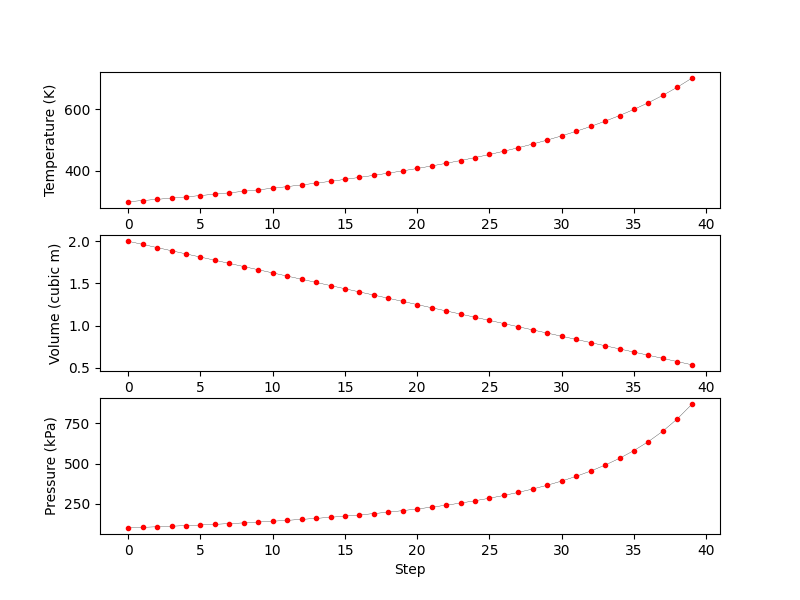
\includegraphics[width=\textwidth]{chunkplot1.png}
    \caption{Chunk plots of temperatures every 40 steps.}
    \label{fig:chunkplot1}
\end{figure}

However, we will get better estimates if we break it up into 400 steps instead of 40. Change the line that defines the number of steps:

\begin{Verbatim}
step_count = 400 # steps
\end{Verbatim}

Now the predicted temperature and pressure should be something like $753.603^\circ$ K and 1004.803 kPa.  (This is much closer to the correct result: :$755.953^\circ$ K and 1007.937 kPa.)

What if you break it into 400,000 steps? Now, the result should be really, really close to correct. And the plot is quite accurate:
\begin{figure}[htbp]
    \centering
    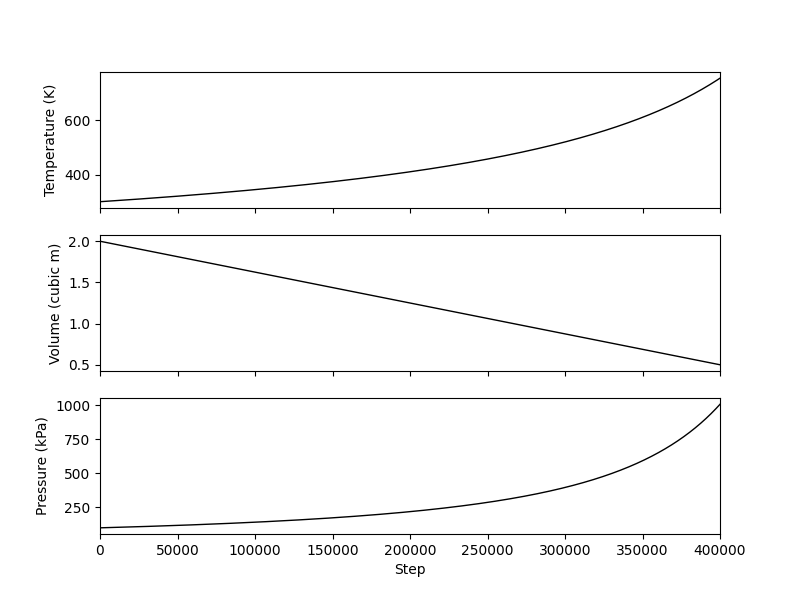
\includegraphics[width=\textwidth]{chunkplot2.png}
    \caption{Chunk plots of temperatures every 400 steps.}
    \label{fig:chunkplot2}
\end{figure}

(You can comment out the lines that make the red dots on the graphs. No
one wants to see 400,000 red dots.)

It is inefficient to have to do long simulations to guess the final temperature and pressure. Fortunately, there are two handy rules you can use to skip this:
\index{adiabatic compression}
\index{adiabatic decompression}
\begin{mdframed}[style=important, frametitle={Adiabatic Compression and Decompression}]

Let 

$$\gamma = \frac{C_{P,m}}{C_{V,m}}$$

In an adiabatic compression or decompression, $P$ and $V$ change, but

$$P \left(V^\gamma \right)$$

stays constant.

Also 

$$T \left(V^{\left( \gamma - 1 \right)} \right)$$

stays constant

\end{mdframed}

For a monoatomic gas:

$$\gamma = \frac{C_{P,m}}{C_{V,m}} = \frac{5}{3}$$

$$\gamma - 1 = \frac{2}{3}$$

Before the compression: 

$$T \left(V^{\left( \gamma - 1 \right)} \right) = 300 \left( 2^{0.6667} \right) = 476.22$$

After the compression it has to be the same:

$$T \left(V^{\left( \gamma - 1 \right)} \right) = T \left( 0.5^{0.6667} \right) = 476.22$$

Thus 

$$T = 755.95^\circ \text{ Kelvin}$$

We can then use the ideal gas law to solve for the final pressure:

$$P = \frac{n R T}{V} = \frac{(80.18)(8.31446)(755.95)}{0.5} = 1007937 \text{ pascals}$$

That is hot! As you let it cool back down to 300 degrees Kelvin, how much heat would be released? 

$$E = C_{V,m} n \Delta T = (12.47)(80.2)(755.95 - 300) \approx 456 \text{ kJ}$$

\section{How an Air Conditioner Works}

Once again, imagine the accordion-like container filled with helium. Let's say you walked it outside and compressed it from 2 cubic meters to 0.5 cubic meters in a vise. The container would get to 755.95 degrees Kelvin. You keep it compressed in the vise, but let it cool down outside. When it gets back to 300 degrees Kelvin, you walk it back inside.

Now, without letting any molecules in or out of the container, you release the vise. The gas is decompressed and gets very cold. How cold? Cold enough to accept about 456 kJ of kinetic energy from your house. That is, it would absorb heat from your house until the gas inside was the same temperature as your house.

So, you walk outside with your accordion and your vise, and repeat:
\begin{enumerate}
\item Compress the gas outside.
\item Let the hot gas cool down outside.
\item Walk the room-temperature compressed gas inside.
\item Decompress the gas inside.
\item Let the cold gas warm up inside.
\end{enumerate}

You could keep your house cool on a hot day this way. This is not unlike how an air conditioner works.

There is a hose filled with refrigerant that does a loop: 
\begin{itemize}
\item Outside, the refrigerant is compressed and allowed to cool to the outside temperature. (Usually there is a big fan blowing on a coil of refrigerant to speed the process.)
Inside, the refrigerant is decompressed and allowed to warm to the inside temperature. (Usually there is a big fan blowing the air of the home past a coil of refrigerant to speed the process.)
\end{itemize}

In each pass of the loop, the refrigerant absorbs some of the kinetic energy from inside the house, and releases it on the outside.

This same mechanism can be used to heat your house. (Units that both heat and cool are known as \newterm{heat pumps}.) 
The heat pump does the process backwards: The hot compressed refrigerant cools down inside. The cold decompressed refrigerant warms up outside.

